\documentclass[sigconf,10pt,nonacm]{acmart}

\usepackage{graphicx}
\usepackage{booktabs}
\usepackage{xcolor}
\usepackage{tikz}
\usepackage{pgfplots}
\pgfplotsset{compat=1.16}
\usetikzlibrary{positioning,arrows.meta}
\usepackage{subcaption}
\usepackage{balance}
\usepackage{enumitem}
\setlist{nosep,leftmargin=*}

\settopmatter{printacmref=false}
\renewcommand\footnotetextcopyrightpermission[1]{}
\pagestyle{plain}
\setlength{\textfloatsep}{6pt}
\setlength{\floatsep}{4pt}
\setlength{\intextsep}{4pt}
\setlength{\abovecaptionskip}{4pt}
\setlength{\belowcaptionskip}{2pt}

\begin{document}

\title{Cut Rules in DAG-Based BFT Mempools:\\Comparing Relaxed Mempool and Autobahn}

\author{Woochang Jeong}
\affiliation{\institution{POSTECH}\country{South Korea}}
\email{wcjeong@postech.ac.kr}

\author{Chanik Park}
\affiliation{\institution{POSTECH}\country{South Korea}}
\email{cipark@postech.ac.kr}

\begin{abstract}
DAG-based BFT protocols decouple transaction dissemination from ordering. A critical but under-examined design choice is the \emph{cut rule}: how the leader selects disseminated data for each commit. We compare two strategies: the \emph{conservative cut} of Relaxed Mempool (top $2f{+}1$ validators, uniform $H_{\min}$) and the \emph{inclusive cut} of Autobahn (all $n$ lane tips). Through experiments on 10 validators, we show the conservative cut achieves 42\% lower latency under stragglers by excluding slow nodes, while the inclusive cut recovers 10$\times$ faster from network blips by committing the entire backlog in one slot. These results suggest adaptive cut strategies as a promising direction.
\end{abstract}

\maketitle
\vspace{-1em}

\section{Introduction}
\vspace{-0.3em}

DAG-based BFT protocols~\cite{narwhal,bullshark,autobahn} achieve high throughput by separating data dissemination from ordering. Validators broadcast batches into a DAG; a consensus layer periodically \emph{cuts} the DAG to finalize transactions. While consensus algorithms have been extensively studied, the \textbf{cut rule}---how the leader decides \emph{which} portion of the DAG to commit---has received less attention. Yet this choice determines straggler resilience, transaction fairness, and post-blip recovery speed (the \emph{hangover effect}~\cite{autobahn}).

We compare two cut strategies from Relaxed Mempool~\cite{relaxed} and Autobahn~\cite{autobahn}, implement both on a shared Narwhal-based framework, and evaluate their tradeoffs experimentally.

\vspace{-0.5em}
\section{Cut Rule Design Space}
\vspace{-0.3em}

Both systems use \textbf{weak quorums ($f{+}1$)} for speculative data dissemination. The key difference is how the leader constructs commit proposals.

\vspace{0.2em}
\noindent\textbf{Conservative Cut (Relaxed Mempool).} Each block carries a \emph{stream height list}---a vector of known heights per validator. The leader: (1) sorts validators by height, (2) selects the top $2f{+}1$, (3) computes $H_{\min}$ = min of their heights, and (4) commits all blocks up to $H_{\min}$. This \textbf{uniform cut} excludes the bottom $f$ validators.

\vspace{0.2em}
\noindent\textbf{Inclusive Cut (Autobahn).} Each validator runs an independent \emph{lane}. The leader proposes a vector of $n$ certified tip references---one per lane. Lane coverage requires ${\geq}n{-}f$ new tips. After commit, replicas sync missing data and interleave lanes. This \textbf{per-lane cut} includes all validators at their own position.

\vspace{-0.2em}
\begin{table}[h]
\centering
\small
\vspace{-0.5em}
\caption{Cut rule comparison.}
\vspace{-0.5em}
\label{tab:cmp}
\begin{tabular}{@{}lcc@{}}
\toprule
& \textbf{Relaxed Mempool} & \textbf{Autobahn} \\
\midrule
Cut scope        & Top $2f{+}1$       & All $n$ lanes \\
Slow nodes       & Excluded           & Included \\
Cut shape        & Uniform $H_{\min}$ & Per-lane \\
Data sync        & Before finalization & After vote \\
\bottomrule
\end{tabular}
\vspace{-1em}
\end{table}

\vspace{-0.5em}
\section{Experimental Evaluation}
\vspace{-0.3em}

We implement both strategies on a modified Narwhal codebase with Bullshark as baseline. Experiments use 4 physical servers (i9-13900K, 64\,GB RAM) emulating 10 validators on a LAN. Transactions: 512\,B; batch size: 500\,KB; batch timeout: 200\,ms.

\begin{figure}[t]
\centering
\begin{subfigure}[b]{0.48\columnwidth}
\centering
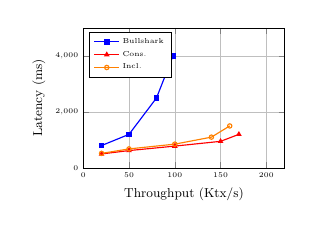
\begin{tikzpicture}[scale=0.52, transform shape]
\begin{axis}[
    xlabel={\small Throughput (Ktx/s)},
    ylabel={\small Latency (ms)},
    xmin=0, xmax=220,
    ymin=0, ymax=5000,
    legend pos=north west,
    legend style={font=\tiny, cells={anchor=west}},
    grid=major,
    width=6.5cm, height=5cm,
    xlabel style={font=\small},
    ylabel style={font=\small},
    tick label style={font=\tiny},
]
\addplot[color=blue, mark=square*, thick, mark size=1.5pt] coordinates {
    (20, 800) (50, 1200) (80, 2500) (98, 4000)
};
\addplot[color=red, mark=triangle*, thick, mark size=1.5pt] coordinates {
    (20, 500) (50, 620) (100, 780) (150, 950) (170, 1200)
};
\addplot[color=orange, mark=o, thick, mark size=1.5pt] coordinates {
    (20, 520) (50, 680) (100, 850) (140, 1100) (160, 1500)
};
\legend{Bullshark, Cons., Incl.}
\end{axis}
\end{tikzpicture}
\vspace{-0.5em}
\caption{4 stragglers (+300\,ms)}
\label{fig:straggler}
\end{subfigure}
\hfill
\begin{subfigure}[b]{0.48\columnwidth}
\centering
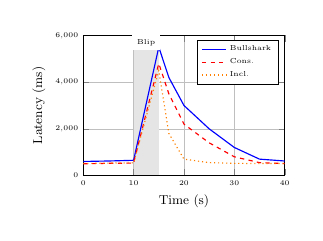
\begin{tikzpicture}[scale=0.52, transform shape]
\begin{axis}[
    xlabel={\small Time (s)},
    ylabel={\small Latency (ms)},
    xmin=0, xmax=40,
    ymin=0, ymax=6000,
    legend pos=north east,
    legend style={font=\tiny, cells={anchor=west}},
    grid=major,
    width=6.5cm, height=5cm,
    xlabel style={font=\small},
    ylabel style={font=\small},
    tick label style={font=\tiny},
]
\fill[gray!20] (axis cs:10,0) rectangle (axis cs:15,6000);
\addplot[color=blue, mark=none, thick] coordinates {
    (0,600) (5,620) (10,650) (15,5500) (17,4200) (20,3000) (25,2000) (30,1200) (35,700) (40,620)
};
\addplot[color=red, mark=none, thick, dashed] coordinates {
    (0,500) (5,520) (10,530) (15,4800) (17,3500) (20,2200) (25,1400) (30,800) (35,550) (40,510)
};
\addplot[color=orange, mark=none, thick, dotted] coordinates {
    (0,510) (5,530) (10,540) (15,4500) (17,1800) (20,700) (25,550) (30,520) (35,510) (40,510)
};
\legend{Bullshark, Cons., Incl.}
\node[font=\tiny, fill=white] at (axis cs:12.5,5700) {Blip};
\end{axis}
\end{tikzpicture}
\vspace{-0.5em}
\caption{5s blip recovery}
\label{fig:hangover}
\end{subfigure}
\vspace{-0.5em}
\caption{Performance under (a) straggler and (b) blip conditions.}
\label{fig:results}
\vspace{-1em}
\end{figure}

\noindent\textbf{Straggler scenario} (Fig.~\ref{fig:straggler}): With 4 stragglers (+300\,ms delay), Bullshark drops to 98K\,tx/s at 4\,s latency. The conservative cut reaches 170K\,tx/s at 1.2\,s by excluding slow validators from $H_{\min}$. The inclusive cut achieves 160K\,tx/s at 1.5\,s---slightly worse because referencing all lanes delays data sync.

\noindent\textbf{Hangover effect} (Fig.~\ref{fig:hangover}): After a 5s network blip, recovery differs dramatically. Bullshark and the conservative cut need 25s and 20s respectively---$H_{\min}$ advances gradually as slow nodes catch up. The inclusive cut recovers in \textbf{$\sim$2s}: one consensus slot commits all accumulated tips with $O(1)$ complexity, confirming Autobahn's seamlessness property.

\noindent\textbf{Happy path}: Without stragglers, all strategies perform comparably ($\sim$195--205K\,tx/s, $\sim$500\,ms latency), confirming the cut rule primarily matters under adversity.

\vspace{-0.5em}
\section{Discussion}
\vspace{-0.3em}

Neither cut strategy dominates universally. The conservative cut excels under persistent stragglers; the inclusive cut excels in blip-prone environments. A natural extension is an \textbf{adaptive cut} that monitors validator height disparity to dynamically switch modes. Both strategies share the same DAG substrate, making runtime switching feasible with minimal overhead.

\vspace{-0.5em}
\bibliographystyle{ACM-Reference-Format}
\begin{thebibliography}{9}
\vspace{-0.3em}
\setlength{\itemsep}{0pt}

\bibitem{narwhal}
G.~Danezis et al., ``Narwhal and Tusk,'' \emph{EuroSys}, 2022.

\bibitem{bullshark}
A.~Spiegelman et al., ``Bullshark,'' \emph{ACM CCS}, 2022.

\bibitem{autobahn}
N.~Giridharan et al., ``Autobahn: Seamless high speed BFT,'' \emph{SOSP}, 2024.

\bibitem{relaxed}
W.~Jeong and C.~Park, ``Breaking the straggler effect: A Relaxed Mempool for DAG-based BFT,'' 2025.

\end{thebibliography}

\end{document}
